\section{Lifted Disjoint Paths}
\label{sec:lifted-disjoint-paths}

The lifted disjoint paths problem is an extension of the node-disjoint paths problem by additional lifted edges that represent connectivity given by the disjoint paths.
They allow to express long-range connectivity priors.

\begin{definition}[Flow Network and Lifted Graph]
Consider two directed acyclic graphs $G = (V, E)$ and $G' = (V',E')$ where $V' =V\backslash \{s,t\}$.
The graph $G=(V,E)$ represents the flow network and we denote by $G'$ the lifted graph.
The two special nodes $s$ and $t$ of $G$ denote source and sink node respectively.
\end{definition}

\begin{definition}[Paths]
We define the set of paths starting at $v$ and ending in $w$ as
\begin{equation}
vw\mhyphen\text{paths}(G) = \{
(v_1v_2,\ldots,v_{l-1}v_l) : \begin{array}{c} v_i v_{i+1} \in E \\ v_1 = v, v_l = w \end{array}
 \}
\end{equation}
For a $vw\mhyphen\text{path}$ $P$ we denote its edge set as $P_E$ and its node
set as $P_V$. 
\end{definition}

\begin{definition}[Lifted Edges]
Given an indicator vector $y \in \{0,1\}^E$ of a node-disjoint set of paths and a lifted edge $e \in E'$ its indicator variable $y'_e \in \{0,1\}$ is defined as
\begin{equation}
\label{eq:lifted-disjoint-paths-lifted-edge}
y'_e \Leftrightarrow \exists P \in vw\mhyphen\text{paths}(G) \text{ s.t. } \forall ij \in P_E : y_{ij} = 1\,.
\end{equation}
\end{definition}

\begin{definition}[Lifted Disjoint Paths Problem]
Given edge costs $c \in \R^E$, node cost $\omega \in \R^V$ for the flow network $G$ and edge costs $c' \in \R^{E'}$ for the lifted graph $G'$ we define the lifted disjoint paths problem as
\begin{equation}
\label{eq:lifted-disjoint-paths}
\begin{array}{cl}
\min\limits_{\substack{y \in \{0,1\}^E, y' \in \{0,1\}^{E'} \\ x \in \{0,1\}^V }} 
&
\la c, y \ra + \la c', y' \ra + \la \omega, x \ra \\
\text{s.t.}
& y \text{ node-disjoint } s,t-\text{flow in } G \\
& x \text{ flow through nodes of } G \\
& y,y' \text{ feasible according to~\eqref{eq:lifted-disjoint-paths-lifted-edge}}\,.
\end{array}
\end{equation}
\end{definition}

An ILP formulation of~\eqref{eq:lifted-disjoint-paths} is given in~\cite{hornakova2020lifted}.
For an illustration of the lifted disjoint paths problem see Figure~\ref{fig:LDP}.

%\begin{figure}[H]
%\centering
%\includestandalone[width=0.8\columnwidth]{figures/lifted-disjoint-paths}
%\caption{
%Illustration of a lifted disjoint paths problem on flow network (black edges) and lifted graph (blue edges).
%Active edges $y,y' = 1$ are solid while inactive edges $y,y' = 0$ are dashed.
%}
%\label{fig:lifted-disjoint-paths}
%\end{figure}

\begin{figure}
	\centering
	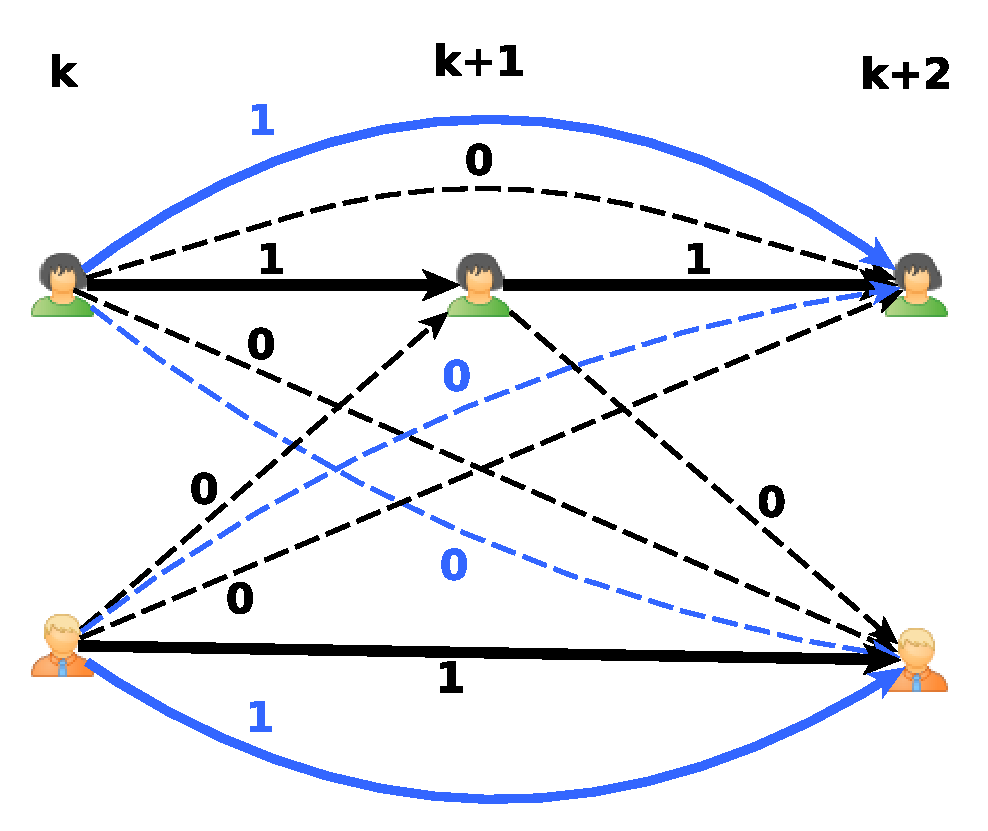
\includegraphics[width=0.9\columnwidth]{images/illustrationLDP}
	\caption{Illustration of a lifted disjoint paths problem on flow network (black edges) and lifted graph (blue edges).
		Active edges $y,y' = 1$ are solid while inactive edges $y,y' = 0$ are dashed.}
	\label{fig:LDP}	
\end{figure}


\subsection{File Format}
\paragraph{File defining costs between pairs of nodes.} Some of the pairs are selected to create flow edges, some of them are selected to create lifted edges according to the strategy for graph creation given by solver parameters. Note that lifted and flow edges can overlap. 
\begin{fileformat}
(*$|V'|$*)
(*$v_1$*),(*$w_1$*),(*$c_1$*)
.
.
.
(*$v_m$*),(*$w_m$*),(*$c_m$*) 
\end{fileformat}
\paragraph{File defining the distribution of nodes in time frames.} Time frames are numbered from $1$ to $T$ (maximal time frame). Nodes are numbered from $0$ to $|V'|-1$. $V_i$ denotes nodes in time frame $i$.
\begin{fileformat}
(*$1$*) (*$0$*)
(*$1$*) (*$1$*)
.
.
.
(*$1$*) (*$|V_1|-1$*)
(*$2$*) (*$|V_1|$*)
.
.
.
(*$2$*) (*$|V_1|+|V_2|-1$*)
.
.
.
(*$T$*) (*$|V'|-1$*)
\end{fileformat}
\paragraph{File with solver parameters.}The file starts with the keyword [SOLVER] (including the brackets). Each parameter name is written with capital letters and underscores. Parameter values follow the $=$ sign.
\begin{fileformat}
[SOLVER]
FIRST_PARAMETER_NAME=value1
SECOND_PARAMETER_NAME=value2
.
.
.
\end{fileformat}

\paragraph{Input file for the approximate solver.} We typically use the same set of parameters for processing all instances within a~dataset. The first LDP solver LifT specifies path to instance files in the parameter file. Therefore, a~separate parameter file is needed for each problem instance. Solver ApLift enables to use one parameter file for multiple instances. The path to instance files and to the parameter file is specified in the input input file that has the following format. 
\begin{fileformat}
INPUT_GRAPH=/path/to/edge/costs
INPUT_FRAMES=/path/to/nodes/in/frames
INPUT_PARAMS=/path/to/parameter/file
\end{fileformat}

\subsection{Datasets}
\subsubsection{MOT Challenge}
The main application of LDP is in multiple object tracking.
The MOT15/16/17 benchmarks \cite{MOTChallenge2015,MOT16} contain semi-crowded videos sequences filmed from a~static or a~moving camera. 
MOT20 \cite{MOTChallenge20} comprises crowded scenes with considerably higher number of  frames  and detections per frame.



\subsection{Algorithms}
\begin{description}
    \item[ILP Solver~\cite{hornakova2020lifted}:] Cutting planes for ILP solvers together with a two-stage procedure for computing tracklets first.
    \item[Message Passing Solver~\cite{hornakova2021making}:] Decompose the full problem into combinatorially solved subproblems and link them together with Lagrange multipliers updated by block coordinate ascent.
\end{description}
